\setcounter{page}{1}
\section{Aufbau und Funktionsweise des Geiger-Müller-Zählrohrs}
\label{sec:aufbau}
Eine schematische Abbildung eines Geiger-Müller-Zählrohrs ist in
Abbildung \ref{fig:geiger} dargestellt.
Es besteht aus einem stählernen Hüllenzylinder mit Radius $r_K$, welcher als
Kathode dient. In der Mitte des Zylinders befindet sich ein Anodendraht mit
Radius $r_a$.
Die Vorderseite des Zylinders ist mit einer für kleine Teilchen
leichtdurchdringbaren Folie (Mylar) versiegelt. Im Inneren des Zählrohrs
befindet sich ein Gasgemisch, zumeist ein Edelgas wie zum Beispiel Argon,
versetzt mit Ethylalkohol. Um das Zählrohr in Betrieb zu nehmen muss eine
Spannung zwischen Kathode und Anodendraht angelegt werden.
\\
Sobald eine äußere Spannung angelegt wird, bildet sich im Inneren ein
radialsymmetrisches E-Feld aus, welches im Abstand $r$ vom Draht die Feldstärke
\begin{equation}
  E(r) = \frac{U}{r\:\ln\left(\sfrac{r_k}{r_a}\right)}
\end{equation}
besitzt.\\
Dringt ein geladenes Teilchen in das Zählrohr, ionisiert es solange die Gasatome,
bis es seine Energie vollständig abgegeben hat.
Haben die Elektronen genug Energie können sie mehr als ein Atom ionisieren und
es kommt zu sogenannten Townsend-Lawinen. Durch die an den Elektroden
auftrefenden geladenen Teilchen und den entstehenden Strom kann auf die
Energie des ursprünglich einfallenden Teilchens geschlossen werden.
Dieser Spannungsbereich wird deswegen auch Proportionalbereich genannt.

Bei höheren Spannungen können UV-Photonen durch Stöße entstehen, diese
elektrisch neutralen Teilchen können sich senkrecht zum Feld ausbreiten und
dort neue Lawinen auslösen, sodass über die Energie keine Aussage mehr gemacht
werden kann, nur noch über die Intensität der einfallenden Strahlung.
Dieses ist der normale Bereich für ein Geiger-Müller-Zählrohr.
Bei höheren Spannungen werden zu viele Lawinen ausgelöst und das Zählrohr kann
daurch zerstört werden.

\begin{figure}
  \centering
  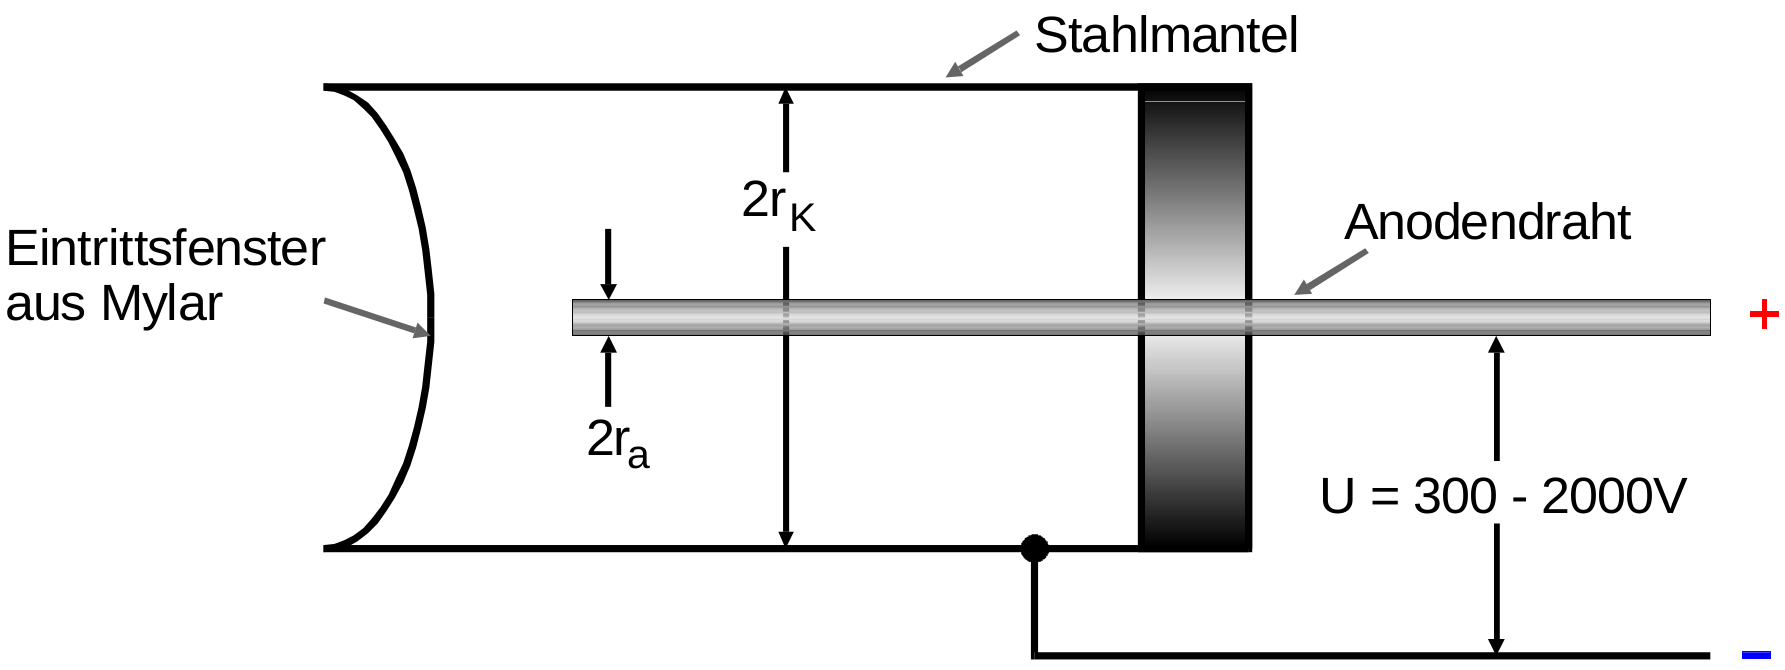
\includegraphics[width=0.65\textwidth]{content/geiger.png}
  \caption{Aufbau eines Geiger-Müller-Zählrohres \cite{Anleitung}.}
  \label{fig:geiger}
\end{figure}
